\subsubsection{Interpreter}
\label{section:perf-interpreter}

The performance of the interpreter with regard to program hotness is shown in \autoref{figure:interpreter-hotness}. From this plot, it is very clear that the interpreter exhibits quite a `flat' performance profile; increasing hotness past a point yields no change in performance. It can be seen however that extremely cold programs do have a lower performance.

\begin{figure}[H]
    \centering
    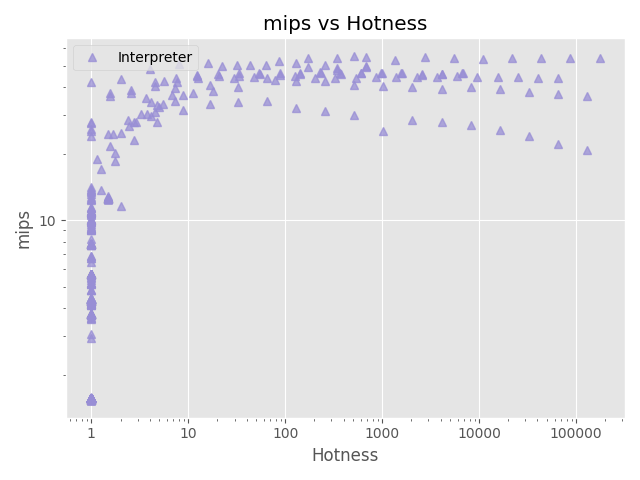
\includegraphics[scale=0.75]{output/graphs/scatter/single/interpreter/hotness.png}
    \caption{Performance (mips) vs hotness for all tests run on the interpreter.}
    \label{figure:interpreter-hotness}
\end{figure}

These results are to be expected; the interpreter is unable to explicitly take advantage of hot blocks as all the work required to emulate a block once is still required for further emulation. Despite this, there are still some savings to be made by executing hotter programs as the (small) initial overheads are amortised. Furthermore, the CPU's branch predictor and cache performance will both increase as the same instructions are emulated more frequently; both of these factors can be attributed to the initial increase in performance as hotness increases.

\autoref{figure:emus-hotness} shows the same relationship between performance and hotness for the interpreter, JIT and hybrid emulators. It can clearly be seen that the JIT and hybrid's performance rapidly increase with program hotness in a manner that the interpreter is simply incapable of. We see that the interpreter is unable to reach or exceed 60 mips under any circumstances. The performance of the interpreter is very consistent and is not as adversely affected by cold programs as the JIT emulator is, however it is also unable to reach a particularly high performance and has a low performance ceiling.

\begin{figure}[H]
    \centering
    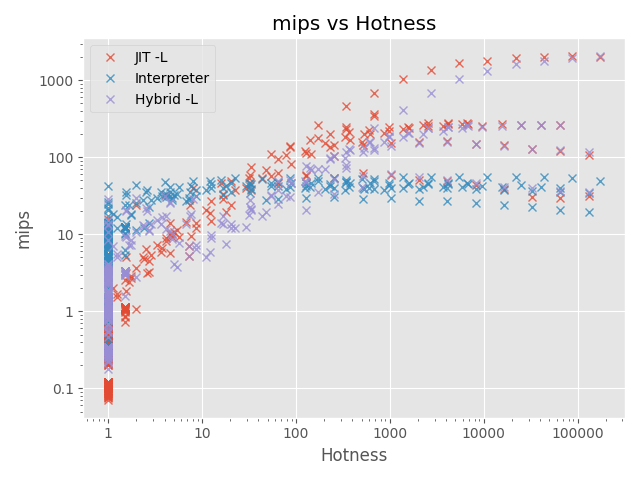
\includegraphics[scale=0.75]{output/graphs/scatter/emulators/hotness.png}
    \caption{Performance (mips) vs hotness for all tests.}
    \label{figure:emus-hotness}
\end{figure}

The interpreter does not contain any configuration options and thus no investigation was required.